% template-v1.tex: LaTeX2e template for Usenix papers.
% Version: usetex-v1, 31-Oct-2002
% Revision history at end.

\documentclass[proof]{usetex-v1}
% Choose the appropriate option:
%
% 1. workingdraft:
%
%       For initial submission and shepherding.  Features prominent
%       date, notice of draft status, page numbers, and annotation
%       facilities.  The three supported annotation macros are:
%               \edannote{text}         -- anonymous annotation note
%               \begin{ednote}{who}     -- annotation note attributed
%                 text                          to ``who''
%               \end{ednote}
%               \HERE                   -- a marker that can be left
%                                               in the text and easily
%                                               searched for later
% 2. proof:
%
%         A galley proof identical to the final copy except for page
%         numbering and proof date on the bottom.  Annotations are
%         removed.
%
% 3. webversion:
%
%       A web-publishable version, uses \docstatus{} to indicate
%       publication information (where and when paper was published),
%       and page numbers.
%
% 4. finalversion:
%
%       The final camera-ready-copy (CRC) version of the paper.
%       Published in conference proceedings.  This doesn't include
%       page numbers, annotations, or draft status (Usenix adds
%       headers, footers, and page numbers onto the CRC).
%
% If several are used, the last one in this list wins
%

%
% In addition, the option "endnotes" permits the use of the
% otherwise-disabled, Usenix-deprecated footnote{} command in
% documents.  In this case, be sure to include a
% \makeendnotes command at the end of your document or
% the endnotes will not actually appear.
%

% These packages are optional, but useful
\usepackage{epsfig}     % postscript figures
\usepackage{url}        % \url{} command with good linebreaks
\usepackage{multirow}
\usepackage{subfig}

\begin{document}

\title{Pomegranate: A Scalable, Efficient Tiny File Store over Tabular Storage}

% document status: submitted to foo, published in bar, etc.
\docstatus{Submitted to EuroSys 2012}

% authors.  separate groupings with \and.
\author{
\authname{Can Ma}
\authurl{\url{macan@ncic.ac.cn}}
\and
\authname{Jin Xiong}
\authurl{\url{xj@ncic.ac.cn}}
\and
\authname{Dan Meng}
\authurl{\url{md@ncic.ac.cn}}
\and
\authaddr{National Research Center for Intelligent Computing Systems}
\authaddr{Institute of Computing Technology, CAS}
\authaddr{Beijing, China, 100190}
} % end author

\maketitle

\begin{abstract}
    The emerging popular Internet applications such as online photo and microblogging services exhibit very different data access and storage requirements from traditional applications. Large number of tiny data are generated, analyzed, and returned every second. Challenging requirements of highly concurrent both high throughput and low latency accesses to tiny files are exhibited.

    In this paper, we propose Pomegranate, a novel distributed file system built over distributed tabular storage, to manage billions of tiny files and support highly concurrent low latency data access. Pomegranate uses extendible hash to index metadata, log-structured storage format and columnar storage to exploit temporal and spatial locality, and snapshot-able and reconfigurable caching to increase parallelism and tolerant failures.

    We present the design and implementation of Pomegranate. Our evaluation results demonstrate that the core tabular storage of Pomegranate can serve linearly increased more than 100,000 aggregate read and write requests per second(RPS) on 82 nodes.
\end{abstract}

\section{Introduction}

    With the popularity of Internet and wireless communications, more and more Internet applications rely on processing large volumes of data to provide services. The Internet applications exhibit very different data access and storage requirements from traditional applications. In addition to storing and accessing petabytes of data efficiently and economically, many such applications need to efficiently support millions to hundreds of millions of on-line users to concurrently access tiny objects with typical size of no more than hundreds of KB. For example, Facebook, a famous social network site, maintained over 60 billions of photos in 2009 and provided a peak throughput of accessing 550K photos per second\cite{facebook-haystack}. Taobao, a famous e-commercial site in China, maintained over 20 billions of photos, and the average photo size is 15KB. Today's telecommunication companies keep billions of conversation records, with the typical size of tens to hundreds of bytes. And geographic information services such as Google Earth rely on billions of satellite images. With more and more emerging applications such as Twitter\cite{twitter} and SNS applications, the requirement for store and access billions of tiny objects is increasing. We can foresee that web applications in the next few years require scalable distributed storage systems that can efficiently store, access, process and analyze on very large data sets, and provide high throughput and low latency access to billions or even trillions of tiny objects. However, traditional distributed file systems as well as parallel file systems cannot meet this requirement, because they are designed to optimize I/O bandwidth of larger-sized data accesses rather than optimize access latency for smaller-sized data accesses. In these file systems, the cost of accessing a small file is very high, because each such access consists of several disk seeks.

    Due to the inefficiency of small file access in traditional distributed file systems, Internet applications have to develop their own storage systems to meet the low latency, consistency, and structured data storage requirements. For example, both Facebook and Taobao developed their customized distributed storage systems Haystack\cite{facebook-haystack} and TFS\cite{taobao-tfs} respectively to efficiently store and retrieve tens of billions of photos. Moreover, Google uses BigTable\cite{bigtable} to provide service of web indexing, Google Earth maps, and Gmail; Yahoo! use PNUTS\cite{pnuts} as their data serving platform for web applications; and Amazon developed Dynamo\cite{dynamo} to serve order requests in e-commerce. All these self-developed storage systems have been proved efficient for these applications to access billions of tiny objects and structured data in recent years' practice. However, these systems have different interfaces and functionalities, which make them difficult to be used by other applications with similar requirements. File access interface is the most popular data storage and access interface that has been widely used by various types of applications for almost 40 years. Our goal is to design a distributed file system to meet these requirements so that a lot of existing applications can take the advantages of this file system without modification.

    Traditional distributed file systems are too heavy and lacking key capabilities to be adopted in the emerging web applications.

    \textbf{Inefficient Metadata Structures:}
    they are designed for high aggregate I/O bandwidth, not for low latency of tiny file accesses, nor for large numbers of concurrent tiny file accesses. In these file systems, directory entry, inode and data of the file are on different locations of the disk. Hence, access a tiny file needs at least 3 disk accesses, and concurrent tiny file accesses turn out to be large numbers of random disk I/O that are very inefficient because of the mechanical part of disks. Meanwhile, file systems always use hash tree or B+ tree for indexing in each directory. These methods are not scalable and efficient for accessing billions of tiny files. Moreover, because of the inability of storing billions of entries in the same directory efficiently, applications are always advised to spread the entries into hierarchical directories. Unfortunately, this approach incurs more overhead in path name lookup.

    \textbf{Not Transparent Scalable:}
    dynamic node changes such as nodes add-in and remove-out may lead to offline of the file system. Node changes in traditional file systems are not transparent to administrators and users. Name space or data have to be reprovisioned by human to exploit the new nodes.

    \textbf{Moderate Caching:}
    user experienced service latency impacts the business popularity. Memory caching can supply remarkable latency reduction and is very important for storage systems for online web services. However, efficient metadata memory organization approach, including memory caching, scalable and fast memory indexes, is not one of the design considerations of traditional file systems. Caching is always used carefully to not compete with user applications.

    In this paper, we introduce Pomegranate, a distributed file system designed to support both high throughput and low latency accesses to billions of tiny files. To achieve this goal, Pomegranate uses a novel design different from traditional distributed file systems. It is built on top of a distributed tabular system called xTable, which is used for managing trillions of tiny files as well as their metadata. Directories in file system are mapped to tables in xTable. Pomegranate adopts four different technologies to accelerate tiny object accesses. 1) It adopts distributed extendible hash\cite{eh} to index the rows by row keys in order to support nearly \emph{zero-hop} name lookup operations for a single directory that contains billions of files. 2) By combining log structure storage format and columnar storage together, it can exploit data locality and sequential writing, which significantly improves the throughput of concurrent tiny file accesses. 3) It adopts reliable asynchronous inter-table updates to reduce latency and keep eventually consistency for file operations such as mkdir and rmdir that need to update more than one tables. 4) It decouples cache and storage to provide snapshot-able and reconfigurable caching layer to increase parallelism and tolerant node failures.

    The main contribution of Pomegranate is that it is a distributed file system built over distributed tabular storage to support highly concurrent accesses to billions of tiny files, and provide both high throughput and low latency. We optimize the tabular storage system for fast and reliable file system metadata management and tiny file access. We revisit traditional file system directory structures and propose a table-like model to organize both memory and storage structures. We propose to decouple caching and storage for scalability. We also explore to integrate the key/value interface into distributed file systems and export it to user applications. Thus, Pomegranate can compete with tabular storage systems such as BigTable, HBase\cite{hbase}, and Cassandra\cite{cassandra} both in performance and in ability.

    The remainder of this paper is organized as follows. Section 2 describes the backgrounds and related works. Section 3 presents the rationale of design considerations. The design and implementation details are presented in Section 4. Section 5 shows the experiment results and analysis. Finally, Section 6 concludes the whole paper.

\section{Related Works}

    To build a distributed file system over tabular storage system and satisfy both high throughput and low latency demands for tiny object access is nontrivial. Although Swapnil Patil et al\cite{hotcloud} has considered to integrate BigTable-like functions into file system, they have not implemented it yet. There are some fundamental issues that should be considered carefully. Firstly, how to store these huge amounts of metadata and tiny files, and query them efficiently? Secondly, is the tabular storage system sufficient for constructing a large scale metadata service?

    \begin{table*}[tbp]
    \centering
    \begin{tabular}{|l|p{.16\textwidth}|p{.25\textwidth}|p{.35\textwidth}|}\hline
    Storage System & Index Structure & Storage Structure & Logical View \\\hline
    Ext3 & hash tree & indirect block tree & 1-D table indexed by name hash \\\hline
    ZFS & extendible hash & 3-level block tree & fast 1-D table indexed by name hash \\\hline
    Ceph & frag tree & fragment mapped to RADOS & fast 1-D table indexed by name hash \\\hline
    GIGA+ & extendible hash indexed partition & partition mapped to native directory & 1-D table partitions indexed by fixed name hash \\\hline
    SkyFS & extendible hash indexed partition & partition mapped to native file & 1-D table partitions indexed by fixed name hash, unsorted list within partition \\\hline
    BigTable & distributed B+ tree & sorted immutable tablets & multi-dimension table indexed by key \\\hline
    HayStack & hash table & log structure store & 1-D table indexed by object id \\\hline
    \end{tabular}
    \caption{Summary of Index and Storage Structures}
    \label{tab-index}
    \end{table*}

    \textbf{Store and Query Billions of Tiny Objects?}
    In Table \ref{tab-index} we summarizes the index and storage structures of directory or table in existing storage systems. We abstract the directory structures in file systems to a logical table with different properties. To store billions of tiny objects quickly, disk I/O should be fully utilized to transfer data to disk. From Table \ref{tab-index}, the storage structures of file systems are complex and could not exploit the locality. Meanwhile, querying on billions of tiny objects needs fast, extendible index structures and memory caching layer. Table \ref{tab-cache} summarize the cache properties of typical storages.

    \textbf{Gaps between File System and Tabular Storage:}
    To build a distributed file system over tabular storage we have to address 4 issues in tabular storage: efficient storage structures, efficient index structures, reliable inter-table updates, and parallel fault tolerant caching.

    Thus, we revisit traditional file systems and emerging storages in detail to find our way.

    \subsection{Storage Structures}

    To accelerate tiny file access, native file systems are fixed by exploiting data locality to eliminate random I/Os. For example, C-FFS\cite{cffs} and Ceph\cite{ceph} embedded the file inode within directory entry to eliminate indirect access in file lookup stage. hFS\cite{hfs} used log structured file format to aggregate tiny files and flushed them as a whole to disk to utilize the sequential I/O bandwidth. BabuDB\cite{babudb} used log structured merge trees to eliminate small random access of metadata operations. Storage structures for tiny files in parallel file systems such as PVFS\cite{pvfs} are fixed either. Michael et al \cite{europar08} had proposed to remove the metafile, which is not needed for tiny files, to increase metadata throughput. Philip et al \cite{ipdps09} had integrated batched metadata commits to exploit I/O bandwidth.

    Tabular storage such as BigTable aggregates tiny objects into a larger-sized sorted table called SSTable. Disk I/O can be utilized efficiently, however, the immutable property of SSTable is not suitable for heavily modifying accesses, for example file system metadata operations. Moreover, cells are versioned and compacted in SSTable. Loading a specific row may need to scan many SSTables. Customized object stores are using to store billions of files and they can achieve \emph{one} I/O seek for each query. For example, Haystack\cite{facebook-haystack} is an object store for serving HTTP image requests. Images are stored as needles (objects) in a log structured storage. Haystack simplifies image metadata to cache them all in memory. Thus, only one seek is needed to load the image from disk. It is a highly customized storage system and applications have to be rewritten to utilize the power of Haystack.

    \subsection{Index Structures}

    Many distributed file systems are trying to solve the problem of management and accesses of billions of files. They give us a perspective on fast tiny file access. The more efficiently we arrange the metadata, the more quickly we access the tiny files. For example, GIGA+\cite{giga} and SkyFS\cite{skyfs} use scalable index structures to construct directories. GIGA+ hashes the name of directory entries extendibly and partitions each directory to a group of servers. SkyFS uses another hash level to enhance the adaptiveness and scalability of GIGA+. However, GIGA+ and SkyFS are not ideal for tiny file access themselves. I/O paths to read and write tiny files are identical to traditional file systems. They are not efficient because of many seeks in the I/O stage. Moreover, GIGA+ and SkyFS store each file data in separate native files. Transforming tiny file access to native file access would introduce several other index lookups and seeks, which increases the latency.

    Tabular storage, key/value store, and object storages arrange data in more structural ways. Tiny objects are arranged as tables, key/value pairs, or indexed objects. To store and query large data set, scalable index structures such as distributed B+ tree, distributed hash table, and consistent hash\cite{ch} are used. Tabular storage such as BigTable has been used to store tiny files in Google Earth and GMail. However, Sean Quinlan said that \emph{``BigTable isn't really ideal for that purpose in that it requires resources for its own operations that are nontrivial''}\cite{gfs}. For example, distributed B+ tree for locating tablet servers leads to several network lookups for every access. Key/value stores are always built on top of distributed hash table\cite{chord}. DHT is scalable but needs O(logN) hops for each query and is not space efficient. Metadata for each key space, for example the entire routing table in Dynamo, has to be spread to each node. Moreover, key/value pairs are uniformly randomized to each node. It is difficult to set up other levels of memory or storage index structures to utilize locality.

    \subsection{Metadata and Data Caching}
    \begin{table*}[tbp]
    \centering
    \begin{tabular}{|l|c|c|c|c|c|}\hline
    Name & Metadata & Data & Cache \& Storage & Online Reconfigurable? & Snapshot-able?\\\hline
    Ext3 & Cached & Cached & Coupled locally & No & No\\\hline
    ZFS & Cached & Cached & Coupled locally & No & Yes\\\hline
    GIGA+ & Cached & Not cached itself & Coupled locally & No & No\\\hline
    Ceph & Cached & Not cached itself & Coupled remotely & Yes & No\\\hline
    BigTable & Cached & Cached or uncached & Coupled remotely & Yes & No\\\hline
    HayStack & Cached & Uncached & - & - & -\\\hline
    Memcached & - & Cached & - & Yes, w/ data loss & No\\\hline
    VoltDB & - & Cached & - & No & -\\\hline
    \end{tabular}
    \caption{Summary of Cache Properties}
    \label{tab-cache}
    \end{table*}

    In Table \ref{tab-cache}, we summarized the cache properties of existing data stores. To access tiny files quickly, metadata and data are tend to be cached in memory. To store billions of tiny files, there must be a server cluster which is failure prone. Caches and storages can be coupled locally or remotely. Remotely coupled caches can tolerant more node failures than locally coupled caches. Node failures can be tolerant by transparently reconfigure the cluster. Unfortunately, file systems in Table \ref{tab-cache} except Ceph are all not capable to tolerant node failures. In memory key/value stores and database such as memcached\cite{memcached} and VoltDB\cite{voltdb} are not capable to transparently tolerant node failures either.

    In ZFS\cite{zfs}, the cached metedata and data are snapshot-able. A memory snapshot is always consistent and can be safely written to disk quickly. Meanwhile, there is no need to keep an operation log, which is always a serial point of request flows, to record modifications. Thus, snapshot-able caching can eliminate serial accesses to increase parallelism and concurrent throughput.

    \subsection{Reliable Inter-table Update}

     Most tabular storages, key/value stores, have no mechanism to propagate updates from one table or keyspace to another reliably. Actually, there is no requirement to do such updates across tables or key spaces. But, mapping file system directory to table would introduce inter-table updates unavoidably. Usra Minor\cite{usraminor}, which adopts key/value store as its metadata service, uses metadata migration to eliminate multisite updates. However, this migration approach is not efficient, because migration incurs high overheads for cross server updates.

\section{Rationale}
\label{sec-rationale}

    \textit{Design Principles of Pomegranate:
    \begin{itemize}
    \item Build global name space over mature distributed file systems to exploit their capability for large files;
    \item Transparently scalable to a large set of machines to exploit the parallelism;
    \item Exploit the locality both in spatial and in temporal;
    \item Exploit the main memory to serve requests with lower latency;
    \end{itemize}
    }

    Many stable and efficient file systems have already solved the problem of providing high I/O bandwidth. We do not want to reinvent the wheel. Therefore, we build Pomegranate with bottom-up approach to stand on the \emph{Shoulders of Giants}. Thus, Pomegranate has the instinct of supporting high I/O bandwidth applications. To manage the combined global name space and billions of tiny objects, Pomegranate is built over tabular store to support large scale metadata management.

    In POSIX file systems, directory table and inode table are always separated to support two different types of lookup. Lookups by pathname are handled by directory table, while lookups by inode number are handled by inode table. It is nontrivial to consistently update these two indexes, especially in a distributed file system. Meanwhile, using two indexes has increased the lookup latency, which is unacceptable for accessing tiny files. Typically, there are in memory caches for dentry and inode, however, these caches cannot easily extend. Modifying metadata has to update multiple locations. To keep consistency, operation log is introduced. While, operation log is always a serial point for request flows. Thus, we introduce table-like directory and new cache layer to overcome these issues.

    \subsection{Table-like Directory Structures}

    To store and query efficiently both in memory and in persistent storage, we propose a flexible table model (showed by Figure \ref{fig-data-model}), named xTable, for file system directories.  Table is indexed by primary keys, which are the hash value of the file name. Each file has a unique identifier, named UUID, and we use UUID as the file inode number. Lookups by file name can be easily served, while lookups by inode number must provide file name hash value to find the location.

    Distributed extendible hash\cite{giga} is used to shard one directory to many servers to exploit parallelism. To manage billions of table slices and minimize memory usage, extendible hash\cite{eh} is used to index the in-memory entries. By combining these structures together, we can achieve both inter-node and intra-node scalability.

    For tiny files, it is efficient to merge data content with metadata to exploit spatial locality. Thus, we use columnar storage to group some co-queried columns (tags or versions in Figure \ref{fig-data-model}) together. Moreover, to exploit temporal locality and promote I/O efficiency, newly committed data and metadata are appended to the storage file sequentially.

    In general, we propose a novel directory structure that is \emph{multi-level extendible hash indexed table combines columnar storage and log structure storage format together}.

    \subsection{Snapshot-able and Reconfigurable Cache Service}

    For many web applications, for example photo store, there is always a hot set. Cache layer is important for low latency access, especially when the access pattern has temporal locality. Traditional file systems use main memory with caution to not compete with user applications. However, for many applications, file system servers are running just for request handling. So, we focus on the cache design to exploit main memory to deliver better performance. Scalable memory structures and parallel access method are introduced.

    For scalability and performance consideration, cache lines are indexed by extendible hash. Even under heavy load, access to the cache is always O(1). The cache is snapshot-able. Modifications are simply applied to the cache and we atomically snapshot the cache layer at specific rate. Each snapshot is local consistent, unchangeable, and committed to storage layer transactionally.

    We also \emph{decouple} cache layer and storage layer. Thus, each layer can easily scale up and down without interfering each other.  Node failures are detected by loss of heartbeats and cache service can be transparently reconfigured by masking the failed nodes without shutting down any living nodes.

\section{System Architecture}

    \begin{figure}[tbp]
    \begin{centering}
    \epsfig{file=paper.doc/hvfs_architecture.eps, width=.5\textwidth}
    \caption{Architecture of Pomegranate}
    \label{fig-architecture}
    \end{centering}
    \end{figure}

    This section presents the architecture of Pomegranate. Pomegranate is a virtual file system which is constructed on top of a collection of other distributed file systems, shown in Figure \ref{fig-architecture}. It manages all the file system metadata and tiny files, while large files are handled by lower level distributed file systems. As described previously, metadata and tiny file services are built over xTable.

    Clients sit in kernel space and implement POSIX interface; AMC (A Metadata Client) sits in user space and provides more flexible data access method for example key/value; MDS (Metadata Server) provides file system metadata access and tiny data access services; Metadata is loaded from storage back-ends, and cached in memory; MDSL (Metadata/Data Storage Layer) provides metadata and tiny data storage service; while R2 server provides services of site management, address management, file system management and consistent hash ring management. Every other component in Pomegranate must register itself with R2 server to get the current view of the file system, including file system name space, active MDSs and MDSLs. The high level interaction of these components is shown in Figure \ref{fig-interaction}.

    \begin{figure}[tbp]
    \begin{centering}
    \epsfig{file=paper.doc/hvfs_interaction.eps, width=.5\textwidth}
    \caption{Pomegranate Component Interactions}
    \label{fig-interaction}
    \end{centering}
    \end{figure}
%
%    In the logical view, shown in Figure \ref{fig-logical-view}, we just build Pomegrnate on top of the xTable system. xTable provides the cache service and storage service, which can be used as the file system metadata service and storage service. Each directory is transformed to a table of xTable and each directory entry is transformed to a row of the table. As a result, we construct the hierarchical namespace of file system by distributed tables. File system metadata updates which across the directories can be transformed to asynchronous updates of xTable.
%
%    \begin{figure}[tbp]
%    \begin{centering}
%    \epsfig{file=paper.doc/hvfs_logical_view.eps, width=.5\textwidth}
%    \caption{Mapping from xTable to Pomegranate}
%    \label{fig-logical-view}
%    \end{centering}
%    \end{figure}
%
    % ����������ݼ��Լ򻯣��Խ�ʡƪ����
    In logical view, Pomegranate maps file system metadata service to xTable cache service, and tiny file storage service to xTable storage service. A file system directory is transformed to a table in xTable, and each directory entry is presented as a table row. In the next subsections, we describe xTable and Pomegranate separately.

    \subsection{xTable}

    Impacted by Google's BigTable, xTable adopts the column-oriented data model, described by Figure \ref{fig-data-model}. Generally, table in xTable is indexed by primary key and can have unlimited columns. Columns can be added and deleted at any time of the table lifecycle. These multi-columns support makes \emph{semantic indexing}\cite{spyglass} easier to implement. Each access should provide specific $\langle$row,column(s)$\rangle$ to find the location. Fixed numbers of table rows and columns are grouped as a table slice, which is loaded to the cache layer for fast accesses. Multiple columns can be grouped as a combined column and store to one file to expolit the co-query locality. Distributed extendible hashing is used to locate the table rows quickly. Moreover, each table slice has an internal hash table for O(1) access in that slice.

    \begin{figure}[tbp]
    \begin{centering}
    \epsfig{file=paper.doc/hvfs_xtable_data_model.eps, width=.5\textwidth}
    \caption{Data Model of xTable}
    \label{fig-data-model}
    \end{centering}
    \end{figure}

    xTable supports billions of tables in the system. Accesses to each table are sharding to a cluster to increase parallelism. Tables can have complex relationships. For example, adding a row to table A may also need to update another row of table B. So, xTable provides an asynchronous multisite inter-table update interface to propagate updates to another table reliably. Base on this interface, it is easily built a distributed file system over xTable. xTable decouples data caching and data storage subsystems to easily scale up and down separately. Adding more nodes to the caching layer can \emph{linearly} improve system performance. After aggregating a bunch of modifications, cache servers do atomic snapshots of the memory image and commit them to storage layers. Two-phase commit is adopted to guarantee data consistency.

    Metadata requests are always served by cache servers, while data requests can be served by cache servers or storage servers based on configuration. For example, tiny file content can be loaded with the metadata to decrease data access latency. The API of xTable includes \texttt{list}, \texttt{create}, \texttt{lookup}, \texttt{update}, and \texttt{delete}. Every operation is atomic and can be issued with a lot of predefined flags and arguments. This simple but powerful API can be used to implement a file system and a key/value store. We address several important issues in the following subsections.

        \subsubsection{Table Location and Indexing}

        Although each table in xTable can have up to $2^{64}$ rows, an access to any row is always O(1). The hash table size is dynamically expanding on inserting new entries. Tables and requests are distributed to all cache servers to exploit system resources and reach high throughput. Under inserting, table slices are automatically split to enable more parallelism.

        Each table has two indexes: one for locating the cache server and the storage server, and the other for locating the precise row. There are two mappings from table slice id(TS) to virtual server id(CS/SS). To provide better load balancing and tolerant node failures, consistent hash is used to map TS to CS/SS. Each table slice has a bitmap region to manage free slots, a fixed sized hash table to index the rows, and lock regions to synchronize concurrent access. Each table row has a unique name or a unique key. This unique identity can be used to match the precise row. The identity is hashed to value V, while conflicts can be resolved by the identity. As shown in Figure \ref{fig-get-itbid}, $V_l$ is used to search in the per table slice hash table for the target row. The hash table can answer whether a row exists or not quickly. Accesses are sharding to different lock entries to reduce lock contention. $V_h$ is used to locate where the table slice is. Extendible hash is used for locating. For example, client computes the table slice id TS by lookup the bitmap with $V_h$. Then, it use TS to search in the consistent hash ring 0 to get the cache server id CS. Finally, the request can be sent to the cache server CS. The request can be served directly if table slice TS has been loaded from the storage server. Otherwise, cache server compute the storage server SS by searching in ring 1 with TS. Storage server responds the load request with the table slice associated with columns optionally. On receiving TS, cache server inserts it to the memory hash table and serves the original request.

        \begin{figure}[tbp]
        \begin{centering}
        \epsfig{file=paper.doc/hvfs_get_itbid.eps, width=.4\textwidth}
        \caption{Locating Cache Server by Key}
        \label{fig-get-itbid}
        \end{centering}
        \end{figure}

        We enhance the original GIGA+ extendible hash in several fields. Firstly, instead of returning bitmap updates to clients on receiving inaccurate requests, cache servers route the requests to decrease latency. The cache server computes the target cache server $TS_n$ and compares with self id $TS_s$. If $TS_n == TS_s$, then it handles the request, otherwise it forwards the request to the next more accurate cache server $TS_n$. The most accurate cache server finally handles the request, and piggybacks the accurate bits of the bitmap with the reply message. Secondly, add and delete cache servers in xTable is easier than doing these operations in GIGA+. Benefit of decoupling cache servers and storage servers, cache servers' changes do not need to move any stored data. The table slices, which should be cached in another server, can just be invalidated (dropped if they are clean or written back if they are dirty). The new server loads the table slices from storage layer on demand. Thirdly, internal memory structures of cache server and storage structures of storage server are tuned for both low latency and high throughput access. More details are described in Section \ref{sec-cache} and \ref{sec-storage}.

        \subsubsection{Bitmap Consistency}
        \label{sec-bitmap}

        Table rows are organized by distributed extendible hash. Table slice is the bucket of extendible hash, while the directory of extendible hash is represented by the bitmap. Each node has to manage a bitmap view of the table. Clients and servers use bitmap to compute the table slice id. Requests are routed to the final accurate server and bitmap updates are returned to clients. Inaccurate bitmap can not affect correctness but may affect performance. In the insert storm, huge amounts of new table slices are produced in separated nodes. The bitmap view of each server may inconsistent. Although these views will be convergent at last, they would lead to looped request routing between servers.

        To overcome the loop forwarding storm under heavy inserts, we have to accelerate the convergence of bitmap views. Simply broadcasting bitmap updates can work, but it cannot scale in a large cluster. A lot of broadcasted bitmap update messages must be another source of the network contention. We use adaptive gossip\cite{gossip} on bitmap to propagate bitmap changes. On detecting many bitmap changes, servers speed up the gossip process to transfer changes to random nodes. If there is little bitmap changes, servers slow down the gossip process. In our test cluster, looped forwards have been decreased for about two orders of magnitude.

        \subsubsection{Snapshot-able Cache Service}
        \label{sec-cache}

        Cache servers form the cache layer and load table slices from storage servers and manages them in their main memory. This memory caching layer can provide low latency access services for upper layer applications.

        All the loaded table slices are hashed into a memory extendible hash table by table UUID and table slice id. The hash table is expanding dynamically on inserting more table slices with preserving the O(1) access property. On reaching the predefined limit of memory, the least recently used table slices would be forced to write back to storage server or just dropped if it is clean.

        \begin{figure}[tbp]
        \begin{centering}
        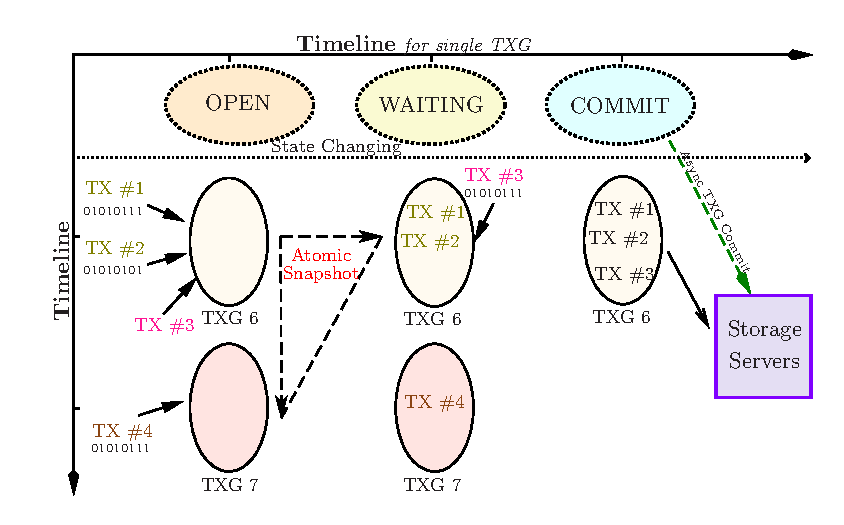
\epsfig{file=paper.doc/hvfs_txg_commit.eps, width=.5\textwidth}
        \caption{Memory Snapshot and Commit}
        \label{fig-txg-commit}
        \end{centering}
        \end{figure}

        Cache servers do not need to log operations requested by clients, even if they are modifications to table rows. Every modification is directly applied to the memory cached table slice. Cache servers aggregate modifications and do atomic consistent memory image snapshot incrementally. Then, the stabilized snapshot can be committed to storage servers as a whole. Copy-on-write is using in the committing phase to minimized memory usage. This group committing mechanism can keep the storage image always consistent in contrast with traditional file systems which log the operations firstly and commit the modifications secondly. Shown by Figure \ref{fig-txg-commit}, on starting a cache server, one commit group is open for absorbing modifications. After several seconds, the opened commit group close and another new group opened for absorbing new modifications. Group changing is an atomic snapshot operation. The closed group waits for the in-progressing modifications and then commits these modifications to several storage servers using two phase commits\cite{2pc}. Dirtied table slices are written back to their target storage servers in parallel to utilize the network bandwidth.

        The table metadata including the table bitmap are managed in another hash table. Even more, there is a write-back bitmap cache which serves bitmap requests from both cache servers and clients. In the bootstrapping phase, cache server gets root table's metadata and bitmap from the central server. Other tables' bitmap and metadata are loaded from cache servers or storage servers automatically.

        \subsubsection{Columnar and Log Structure Store}
        \label{sec-storage}

        Storage layer serves write-back of memory snapshots from cache layer, I/O read/write from clients or cache servers, and table slice reads from cache servers. In this section, we describe the storage strategies adopted in storage layer.

        Table slices written back within snapshots are firstly written to a per-table \emph{append-only} file store to exploit temporal locality. The sequential writing pattern of log structure (append-only) file store can utilize the disk I/O bandwidth maximally. Only in commit phase, the metadata file is updated to point to the newly written table slices. Note that, all the table slices are written to new locations, which means that the old table slices are not overwritten. A partial written snapshot does not introduce any inconsistency. Thus, for all tables in xTable, their storage images are always consistent.

        \begin{figure}[tbp]
        \begin{centering}
        \epsfig{file=paper.doc/hvfs_storage.eps, width=.4\textwidth}
        \caption{Storage Structures}
        \label{fig-xtable-storage}
        \end{centering}
        \end{figure}

        Shown by Figure \ref{fig-xtable-storage}, each table has an individual directory in the host file system. The file `md' records table metadata, for example ranges of table slices this server in charge of. The file `range-*' saves pointers to table slices. The file `TSS' saves the actual table slices, while file `CS.*' saves the combined column data. Indexes to column data are saved in table slices. These metadata files are mmapped to memory on demand for fast access. The last portion of file `TSS' and `CS.*' are mmapped to memory. Table slices and data are \emph{aggregated} in that region to form a large chunk and then written to disk to fully utilize the I/O bandwidth.

        \subsubsection{Reliable Multisite Update}

        Reliable multisite update (RMU), which provides a fast, eventually consistent, and asynchronous update service, is the core function of xTable. Submitted remote updates must be committed to storage layer firstly. Then, they are transferred to target site, processed by the remote RMU in memory, and committed to storage layer at last. Next, the remote RMU replies an OK message. Finally, the original site logs the reply. Incomplete updates are recovered from logs. Although this protocol needs many steps and the whole procedure may last for dozens of seconds, updates in memory can be done quickly, and upper layer applications do not need to block for the commit confirmation. Node crashes in multisite update can be recovered by the commit log. All the unacknowledged updates must be checked and redone. For the efficiency of recovery, a copy of unacknowledged updates are kept in memory, which can provide fast node rejoin after node restart.

        Many xTable internal functions are built with RMU, for example, table slice split and table bitmap update. Table slice split may involve two different sites. The original site transfers the new split table slice to remote site after having committed it to storage layer. RMU transmits the table slice and logs the updates at both original and target site. On failures, splits are either recovered from storage layer or redone with the log. For table bitmap updates, after committing each snapshot a bitmap delta list is traveled and all the bitmap deltas are submitted to RMU to update remote bitmaps quickly and reliably. Moreover, RMU interface is exported to upper layers. For example, Pomegranate uses RMU to implement parent directory updates in mkdir and rmdir. In mkdir, metadata of parent directories must be updated to reflect changes. Mkdir can complete quickly by just submitting the delta update(e.g. `nlink +1'), and the update is guaranteed to reach the parent directory eventually.

        \subsubsection{Fault Tolerance and Data Reliability}

        There is a central server in xTable to provide services such as site registration, management of root tables, consistent hash rings, and site addresses. Every client, cache server and storage server has to register itself to enter the xTable system. In the register phase, each site gets the current view of xTable system. This single server could be the single-point-of-failure. Crash of this server may force the entire system unavailable. We plan to replicate the service to a few servers using Paxos\cite{paxos} (e.g. Zookeeper\cite{zookeeper}) to improve the reliability in the future.

        All the registered sites send heartbeat messages to central server every several minutes. On losing a heartbeat, central server sets the corresponding site state to transient failure and waits for next heartbeat. After a few heartbeat lost, central server pushes the site state to error and trigger the recover process or notify administrator.

        At the storage layer, the data of every virtual site is replicated to another two sites based on consistent hash ring. Each virtual site represents as an Merkle tree\cite{merkle}, and it is monitored by external tools to sync the updates to replicas in incremental manner. The monitor can delay the synchronization by trading-off server load and data reliability.

    \subsection{Pomegranate}

    Management of metadata and tiny files of Pomegranate is built over xTable to utilize distributed tabular storage to provide scalable, low latency and high throughput tiny file access service with POSIX I/O interface. Traditional file system namespace, which is always a hierarchal tree, is transformed to tables with predefined relationships. Moreover, inter-nodes of the hierarchal tree are flatten to a global directory table (GDT) by transforming each directory to a table row. Shown by Figure \ref{fig-namespace-mapping}, each directory is transformed to a GDT entry and a table. All the tables construct the hierarchal namespace and support lookups with pathname. GDT table supports O(1) directory lookups with UUID, and is used in key/value accesses.

    \begin{figure}[tbp]
    \begin{centering}
    \epsfig{file=paper.doc/hvfs_namespace_mapping.eps, width=.5\textwidth}
    \caption{Flatten Hierarchal Namespace to Tables}
    \label{fig-namespace-mapping}
    \end{centering}
    \end{figure}

    As described in Section \ref{sec-rationale}, there are always two separated indexes in POSIX file systems. In Pomegranate, there is only one index that supports both file name lookups and inode number lookups. File names are hashed and each file maps to a table row with a unique identifier UUID. Name hash is used to locate one row, and lookups are corrected by either file name or UUID.

    Simple file system operations such as lookup, create, symlink, unlink, setattr, and getattr, can map to one xTable operation. Complex operations such as hard link and rename, need two or more xTable operations. A standalone transaction server is used to group xTable operations together as a transaction to success or fail. Transaction server could be the bottleneck on processing these operations. Fortunately, these operations are relatively rare with respect to other operations. Operations such as mkdir, rmdir also need two or more xTable operations, but we have tuned them to keep consistency without the transaction server. For example, in mkdir, a table row is created in the parent table firstly, and copied to the GDT table. The table row is recopied on demand in a lookup operation if it hasn't been copied yet because of node failures.

    VFS operations are relayed to Pomegranate or other deployed distributed file systems. Tiny file access and metadata access are served by MDS servers. Large file I/O access is relayed to other distributed file systems. We have implemented a key/value interface for accessing Pomegranate. The interface includes \texttt{list} key-space, \texttt{put}, \texttt{get}, \texttt{update}, and \texttt{delete} key/value pairs. Using this interface can get not only better performance but also distributed storage-edge executions. For example, predicate of substring match is integrated into storage servers. User can issue queries such as ``\textbf{select} * \textbf{from} table \textbf{where} `xyz' \textbf{in value}'' to get all the keys whose value contain substring `xyz'.

    Meanwhile, Pomegranate provides client transactions to guarantee specific operations to hit stable storage. Every transaction is logged at the client firstly. Crash of MDS can be recovered and the pending transactions would be redone. Transaction has \emph{replied} and \emph{committed} stages. User requests are satisfied in replied stage to decrease latency, while the transaction is still ongoing to committed stage.

    We support multiple file system instances running in the same server pool. Each instance is addressed by unique fsid. File system metadata, such as created files and used bytes, are spread to cache servers. The current value of these variables are both committed to storage layer and sent to R2 server within heartbeat messages. Abnormal shutdown or node failures triggers the node recovery process to get the newest metadata.

\section{Performance Evaluation}

    \begin{table}[tbp]
    \centering
    \begin{tabular}{|l|p{.13\textwidth}|l|r|}\hline
    \multicolumn{2}{|c|}{Hardware} & \multicolumn{2}{|c|}{Software}\\\hline
    CPU & 1 1.6GHz Intel Xeon, 4 Core & Kernel & 2.6.16.20\\\hline
    Memory & 4 GB & Glibc & 2.4\\\hline
    Network & Giga Ethernet & fio & 1.22\\\hline
    \multirow{4}{*}{Disk} & \multirow{4}{.13\textwidth}{ST31000524NS SATA, 1TB, 7200RPM} & Seq Write & 42.15 MB/s\\
    & & Seq Read & 59.12 MB/s\\
    & & Rnd Write & 682 IOPS\\
    & & Rnd Read & 3812 IOPS\\\hline
    \end{tabular}
    \caption{Configuration and Disk Perf. of the Test Cluster}
    \label{tab-configuration}
    \end{table}

    We deploy and evaluate Pomegranate on a medium scale cluster (82 nodes), and analyze the results. The hardware, software configuration and I/O performance of the disk of each node are described in Table \ref{tab-configuration}.

%    \subsection{xTable Performance}

%        \begin{table*}[tbp]
%        \centering
%        \begin{tabular}{|p{.1\textwidth}|p{.1\textwidth}|p{.15\textwidth}|p{.1\textwidth}||p{.2\textwidth}|p{.2\textwidth}|}\hline
%        Operation & Aggregated Time(s) & Wall Time(s)$ _{slowest}$ & Stdev of Wall Time & {\textbf{RPS}} $ _{lower\ limit}$ & Average {\textbf{Latency}}(us)\\\hline
%        create & 13101 & 173 & 12.44 & 947,922 & 79.89 \\\hline
%        lookup & 14588 & 191 & 15.66 & 858,549 & 88.95 \\\hline
%        lookup,write data,update metadata & 38052 & 670.2 & 32.55 & 244,703 & 232.03 \\\hline
%        lookup,read data & 124075 & 1547 & 9.79 & 106,010 & 756.55 \\\hline
%        delete & 14081 & 185 & 14.66 & 886,391 & 85.86\\\hline
%        \end{tabular}
%        \caption{API Performance of xTable}
%        \label{tab-performance}
%        \end{table*}

        For now, our kernel level client is not mature and under heavy optimization. We measure the performance of the core of Pomegranate by running a series of micro-benchmarks, which adopt the xTable API, to create files, lookup files, write data, read data, and delete files. In the experiment, we use \emph{write-through} data cache and dynamic snapshot interval. Snapshot and commit are delayed to when the load is low or a snapshot timeout occurs to absorb more modifications. Thus, there is almost no commit I/O and COWed table slices in the create and delete stages. Tiny file length is randomly generated in byte range [0,1000). We run the test cases on 82 nodes: each node runs one MDS server, one MDSL server, and one client. Each client does 2,000,000 operations in the \emph{same} directory with 160 threads. Thus, after creating, we have got 164 million files in one directory. Table \ref{tab-performance} shows results of the test cases: xTable achieves amazing aggregate RPSs (Request per Second) on heavily  modifying load. Note that we have not synchronized the execution of clients among nodes, but we have synchronized the execution of threads in each node.

        \begin{table}[tbp]
        \centering
        \begin{tabular}{|c|r|r|r|}\hline
        & Wall Time &  \textbf{RPS} & Average \\
        Operation & (s) $ _{slowest}$ & $ _{lower\ limit}$ & \textbf{Latency} \\\cline{2-2}
        & $ _{stdev}$ & & (us) \\\hline
        \multirow{2}{*}{create} & 173 & \multirow{2}{*}{947,922} & \multirow{2}{*}{79.89} \\\cline{2-2}
        & 12.44 & & \\\hline
        \multirow{2}{*}{lookup} & 191 & \multirow{2}{*}{858,549} & \multirow{2}{*}{88.95} \\\cline{2-2}
        & 15.66 & & \\\hline
        lookup, & \multirow{2}{*}{670.2} & \multirow{3}{*}{244,703} & \multirow{3}{*}{232.03}\\
        write data, & & & \\\cline{2-2}
        update metadata & 32.55 & & \\\hline
        lookup, & 1547 & \multirow{2}{*}{106,010} & \multirow{2}{*}{756.55}\\\cline{2-2}
        read data & 9.79 & & \\\hline
        \multirow{2}{*}{delete} & 185 & \multirow{2}{*}{886,391} & \multirow{2}{*}{85.86}\\\cline{2-2}
        & 14.66 & & \\\hline
        \end{tabular}
        \caption{API Performance of xTable}
        \label{tab-performance}
        \end{table}

        \textbf{File Create, Lookup, and Delete}

%        \begin{figure*}[tbp]
%        \begin{centering}
%        \epsfig{file=paper.doc/pic/paper.create.eps, width=.5\textwidth}
%        \caption{RPS, Net Utilization, Table Slice Split, and Request Forwards in Create Process}
%        \label{fig-create}
%        \end{centering}
%        \end{figure*}
%
%        \begin{figure*}[tbp]
%        \begin{centering}
%        \epsfig{file=paper.doc/pic/paper.lookup.unlink.eps, width=.5\textwidth}
%        \caption{RPS, Net Utilization in Name Lookup and File Deletion Process}
%        \label{fig-lookup-unlink}
%        \end{centering}
%        \end{figure*}
        \begin{figure*}[tbp]
        \centering
        \subfloat[Create Process]{\label{fig-create}\epsfig{file=paper.doc/pic/paper.create.eps, width=.5\textwidth}}
        \subfloat[Name Lookup and File Deletion Process]{\label{fig-lookup-unlink}\epsfig{file=paper.doc/pic/paper.lookup.unlink.eps, width=.5\textwidth}}
        \caption{Profile of File Create, Name Lookup, and File Deletion Process}
        \end{figure*}
        \begin{figure*}[tbp]
        \centering
        \subfloat[Write RPS, and I/O Bandwidth]{\label{fig-write}\epsfig{file=paper.doc/pic/paper.iow.eps, width=.5\textwidth}}
        \subfloat[Read RPS, and I/O Bandwidth]{\label{fig-read}\epsfig{file=paper.doc/pic/paper.ior.eps, width=.5\textwidth}}
        \caption{Profile of Read and Write Process}
        \end{figure*}
        \begin{figure*}[tbp]
        \begin{centering}
        \subfloat[Impact of Varying Nodes on RPS and Latency]{\label{fig-rps}\label{fig-latency}\epsfig{file=paper.doc/pic/paper.rps.eps, width=.5\textwidth}}
        \subfloat[Impact of Bitmap Gossip in Create Process]{\label{fig-gossip}\epsfig{file=paper.doc/pic/paper.gossip.eps, width=.5\textwidth}}
        \caption{Impacts of Varying Nodes and Bitmap Gossip}
        \end{centering}
        \end{figure*}

%        \begin{figure}[tbp]
%        \centering
%        \subfloat[Aggregated RPS]{\label{fig-rps}\label{fig-latency}\epsfig{file=paper.doc/pic/paper.rps.eps, width=.45\textwidth}}
%        \subfloat[Request Latency]{\epsfig{file=paper.doc/pic/paper.latency.eps, width=.45\textwidth}}
%        \caption{Impact of Varying Nodes on Aggregate RPS and Request Latency}
%        \end{figure}

        Create zero-length files only modify the metadata. Our experiment client issues multiple create requests in parallel. For each directory, there are default 8K slots free to create. Beyond this threshold, load is dynamically spread to other nodes to exploit more resources. Because of the hash function, file creates are naturally load balanced across cache servers. From Figure \ref{fig-create} we find that create RPS is highly related to the split rate. This result shows the expected effect of table slice split. The more slices are split, the more parallelism and performance we can get. The experiment also shows that only at startup stage split table slices are transferred to remote nodes to exploit more node resources. Then they are tend to split in the same node. We also note that the number of table slices are increased steadily with creates. At the startup stage (before 50s), a lot of requests are forwarded, while half of them are loop forwarded. By gossiping the bitmap, we have already decreased the looped forwards for two orders of magnitude. While bitmap can't be gossiped to clients, so there are always incorrect requests need to be routed to correct servers throughout execution.

        Name lookup and file delete are simple metadata operations. At 450s, the bitmap is not stabilized yet. Thus, there are a little requests routed in Figure \ref{fig-lookup-unlink}. While, after 3800s, the bitmap is stabilized and there is no requests routed. We have got lower RPS for lookup and delete RPS than create in 82 nodes test. However, we have observed that in other tests lookup and delete RPS are always higher than create.

        \textbf{Write and Read Tiny Files}

%        \begin{figure*}[tbp]
%        \begin{centering}
%        \epsfig{file=paper.doc/pic/paper.iow.eps, width=.5\textwidth}
%        \caption{Write RPS, and I/O Bandwidth}
%        \label{fig-write}
%        \end{centering}
%
%        \begin{centering}
%        \epsfig{file=paper.doc/pic/paper.ior.eps, width=.5\textwidth}
%        \caption{Read RPS, and I/O Bandwidth}
%        \label{fig-read}
%        \end{centering}
%        \end{figure*}

        In our experiment, clients issue parallel file write requests. The length of tiny files is in range [0, 1000B). The total size of these files is 100.5GB. From Table \ref{tab-performance}, average IOPS for each node is 2984, which is \emph{four} times of the IOPS of random writes (from Table \ref{tab-configuration}). This is the expect result, because we transform random file writes to sequential file appends. Figure \ref{fig-write} shows instant RPS and I/O bandwidth in the write stage. The reason of RPS decreased along with execution is that threads had completed their execution gradually and the total load is lower. Below the RPS threshold, memory snapshot is triggered and committed to storage layer. Thus, I/O bandwidth and number of COWed table slices increased after 1400s.

        Tiny file read is very difficult to transform to sequential read. Both requests issued by clients and requests handled by MDSL are randomized. For each file read, we do our best to serve it with merely one I/O access. As a result, shown by Figure \ref{fig-read}, the average IOPS for each node is 1293. This result is not as good as the IOPS of random reads in Table \ref{tab-performance}, but we expect a performance promotion after adopting the asynchronous I/O model.

        \textbf{Linear Scalability}

%        \begin{figure}[tbp]
%        \begin{centering}
%        \epsfig{file=paper.doc/pic/paper.rps.eps, width=.5\textwidth}
%        \caption{Impact of Varying Nodes on Aggregated RPS}
%        \label{fig-rps}
%        \end{centering}
%        \end{figure}
%
%        \begin{figure}[tbp]
%        \begin{centering}
%        \epsfig{file=paper.doc/pic/paper.latency.eps, width=.5\textwidth}
%        \caption{Impact of Varying Nodes on Latency}
%        \label{fig-latency}
%        \end{centering}
%        \end{figure}

        Next, we examined the impact of number of nodes on RPS and latency. Each node issues 2,000,000 requests for create, lookup, and delete operations. On increasing the number of nodes, we not only get more CPU and memory resource, but also get higher load. Our experiment shows that by adding more nodes, the aggregate RPS increased \emph{linearly}. For example, Figure \ref{fig-rps} shows that the aggregated RPS of our system is tend to be linear with the number of nodes. However, latency increases linearly either because of resource contention. Shown by Figure \ref{fig-latency}, the latency of create, lookup, and delete operations are tend to be linear with number of nodes.

        \textbf{Impact of Bitmap Gossip}

%        \begin{figure}[tbp]
%        \begin{centering}
%        \epsfig{file=paper.doc/pic/paper.gossip.eps, width=.5\textwidth}
%        \caption{Impact of Bitmap Gossip in Create Process}
%        \label{fig-gossip}
%        \end{centering}
%        \end{figure}

        To evaluate the impact of gossip on request routing, we run two different tests. The first one run creates on 82 nodes without gossip; while the second one run the same test with gossip. As shown in Figure \ref{fig-gossip}, without gossip there are a lot of forwarded requests and almost all of them are loop forwarded requests, which consume the network bandwidth hungrily. While, with gossip bitmap converges more quickly and loop forwarded requests decreased about two orders of magnitude. Thus, gossip is an efficient way to overcome the inconsistency of bitmap and accelerate the bitmap convergence.

%    \subsection{File System Performance}

\section{Conclusions and Future Work}

This paper presented Pomegranate, a distributed file system that is built over tabular storage. Pomegranate is novel in three key ways: 1) built a global name space and separate I/O path for large files and tiny files, 2) built over tabular storage and mapping file system directory to huge table to manage large numbers of files efficiently(nearly zero hop locating), and 3) built scalable caching and storage layer which are always consistent and reliable. Our experiment shows that the aggregated RPS of Pomegranate increases linearly with adding more nodes.

So far we've focused on the quality of core functions of Pomegranate. As future work, we plan to test the kernel client, dynamically reconfiguration, and fault tolerant support. Also we have already supply a key/value interface for user applications, and on our roadmap we want to evaluate and compare it with other key/value stores. We also want to expose a useful user level API for writing plugins to filter on readdir-like range queries. Even more, we expect file systems can be easily extend with semantic indexing by combining file system and separated indexes (by using xTable).


\section{Acknowledgments}

% This is where the endnotes (see the ``footnote'' above)
% are filled in.  Use this only if you have endnotes.
% \ifhasendnotes\makeendnotes\fi

\begin{thebibliography}{99}

\bibitem{facebook-haystack} Peter Vajgel, \emph{Needle in a haystack: efficient storage of billions of photos}, \url{http://www.facebook.com/note.php?note_id=76191543919}, (2009).

\bibitem{taobao-tfs} Wensong Zhang, \emph{Taobao File System}, \url{http://rdc.taobao.com/blog/cs/?p=128}, (2010).

\bibitem{voltdb} Mike Stonebraker, \emph{VoltDB: the Fast, Scalable Open-Source DBMS}, \url{http://voltdb.com/}, (2010).

\bibitem{zfs} \emph{ZFS: the last word in file systems}. Sun Microsystems. September 14, (2004).

\bibitem{gossip} Andr�� Allavena, Alan Demers and John Hopcroft, \emph{Correctness of a Gossip-based Membership Protocol}, Proc. 24th ACM Symposium on Principles of Distributed Computing (PODC 2005).

\bibitem{2pc} Philip A. Bernstein, Vassos Hadzilacos, Nathan Goodman, \emph{Concurrency Control and Recovery in Database Systems}, Chapter 7, Addison Wesley Publishing Company, ISBN 0-201-10715-5 (1987)

\bibitem{ch} Karger, D.; Lehman, E.; Leighton, T.; Panigrahy, R.; Levine, M.; Lewin, D., \emph{Consistent Hashing and Random Trees: Distributed Caching Protocols for Relieving Hot Spots on the World Wide Web}, Proceedings of the Twenty-ninth Annual ACM Symposium on Theory of Computing, (1997)

\bibitem{paxos} Lamport, Leslie,  \emph{The Part-Time Parliament}, ACM Transactions on Computer Systems 16 (2): 133�C169.(May 1998)

\bibitem{usraminor} Shafeeq Sinnamohideen, Raja R. Sambasivan, Likun Liu, James Hendricks, Gregory R. Ganger., \emph{A transparently-scalable metadata service for the Ursa Minor storage system}, In proceedings of the 2010 USENIX Annual Technical Conference, (USENIX ATC 2010)

\bibitem{bigtable} Chang, Fay and Dean, Jeffrey and Ghemawat, Sanjay and Hsieh, Wilson C. and Wallach, Deborah A. and Burrows, Mike and Chandra, Tushar and Fikes, Andrew and Gruber, Robert E., \emph{Bigtable: a distributed storage system for structured data}, Proceedings of the 7th USENIX Symposium on Operating Systems Design and Implementation, (OSDI 2006)

\bibitem{cassandra} Lakshman, Avinash and Malik, Prashant, \emph{Cassandra: a decentralized structured storage system}, SIGOPS Oper. Syst. Rev. vol 44, 35 - 40, (2010)

\bibitem{pnuts} Cooper, Brian F. and Ramakrishnan, Raghu and Srivastava, Utkarsh and Silberstein, Adam and Bohannon, Philip and Jacobsen, Hans-Arno and Puz, Nick and Weaver, Daniel and Yerneni, Ramana, \emph{PNUTS: Yahoo!'s hosted data serving platform}, Proc. VLDB Endow., vol 1, 1277 - 1288, (VLDB 2008)

\bibitem{dynamo} DeCandia, Giuseppe and Hastorun, Deniz and Jampani, Madan and Kakulapati, Gunavardhan and Lakshman, Avinash and Pilchin, Alex and Sivasubramanian, Swaminathan and Vosshall, Peter and Vogels, Werner, \emph{Dynamo: amazon's highly available key-value store}, Proceedings of twenty-first ACM SIGOPS symposium on Operating systems principles, (SOSP 2007)

\bibitem{hotcloud} Patil, S., G.A. Gibson, G.R. Ganger, J. Lopez, M. Polte, W. Tantisiriroj, L. Xiao, \emph{In Search of an API for Scalable File Systems: Under the table or above it?}, USENIX Workshop on Hot Topics in Cloud Computing, (HotCloud 2009)

\bibitem{eh} Fagin, Ronald and Nievergelt, Jurg and Pippenger, Nicholas and Strong, H. Raymond, \emph{Extendible hashing---a fast access method for dynamic files}, ACM Trans. Database Syst., vol 4, 315 - 344, (1979)

\bibitem{cffs} Ganger, Gregory R. and Kaashoek, M. Frans, \emph{Embedded inodes and explicit grouping: exploiting disk bandwidth for small files}, Proceedings of the annual conference on USENIX Annual Technical Conference, (USENIX ATC 1997)

\bibitem{ceph} Weil, Sage A. and Brandt, Scott A. and Miller, Ethan L. and Long, Darrell D. E. and Maltzahn, Carlos, \emph{Ceph: a scalable, high-performance distributed file system}, Proceedings of the 7th symposium on Operating systems design and implementation, (OSDI 2006)

\bibitem{hfs} Zhang, Zhihui and Ghose, Kanad, \emph{hFS: a hybrid file system prototype for improving small file and metadata performance}, Proceedings of the 2nd ACM SIGOPS/EuroSys European Conference on Computer Systems 2007, (EuroSys 2007)

\bibitem{giga} Swapnil Patil, Garth Gibson, \emph{GIGA+ : Scalable Directories for Shared File Systems}, Carnegie Mellon University Parallel Data Lab Technical Report CMU-PDL-08-110, (2008)

\bibitem{skyfs} Xing, Jing and Xiong, Jin and Sun, Ninghui and Ma, Jie, \emph{Adaptive and scalable metadata management to support a trillion files}, Proceedings of the Conference on High Performance Computing Networking, Storage and Analysis, (SC 2009)

\bibitem{memcached} Fitzpatrick, Brad, \emph{Distributed caching with memcached}, Linux J., (2004)

\bibitem{gfs} McKusick, Marshall Kirk and Quinlan, Sean, \emph{GFS: Evolution on Fast-forward}, ACM Queue, vol 7, 10-20, (2009)

\bibitem{chord} Stoica, Ion and Morris, Robert and Karger, David and Kaashoek, M. Frans and Balakrishnan, Hari, \emph{Chord: A scalable peer-to-peer lookup service for internet applications}, Proceedings of the 2001 conference on Applications, technologies, architectures, and protocols for computer communications, (SIGCOMM 2001)

\bibitem{babudb} J. Stender, B. Kolbeck, M. Hogqvist, F. Hupfeld, \emph{BabuDB: Fast and Efficient File System Metadata Storage}. 6th IEEE International Workshop on Storage Network Architecture and Parallel I/Os,  (SNAPI 2010)

\bibitem{spyglass} Andrew Leung, Minglong Shao, Timothy Bisson, Shankar Pasupathy, Ethan L. Miller, \emph{Spyglass: Fast, Scalable Metadata Search for Large-Scale Storage Systems}, Proceedings of the 7th USENIX Conference on File and Storage Technologies, (FAST 2009)

\bibitem{pvfs} Ligon, III, W.B., and Ross, R. B., \emph{PVFS: Parallel Virtual File Syste}, Beowulf Cluster Computing with Linux, Thomas Sterling, editor, pages 391-430, MIT Press, November, (2001).

\bibitem{europar08} Michael  Kuhn, Julian  Kunkel, Thomas  Ludwig, \emph{Directory-Based Metadata Optimizations for Small Files in PVFS}, Proceedings of the 14th international Euro-Par conference on Parallel Processing, (EuroPar 2008)

\bibitem{ipdps09} Philip Ross Carns, Sam  Lang, Robert Ross Kunkel, Thomas  Ludwig, \emph{Small File Accesses in Parallel File Systems}, IPDPS, (2009)

\bibitem{merkle} Ralph C. Merkle, \emph{A Digital Signature Based on a Conventional Encryption Function}, Conference on the Theory and Applications of Cryptographic Techniques on Advances in Cryptology, (1987)

\bibitem{hbase} HBase, \url{http://hbase.apache.org}, (2010)

\bibitem{zookeeper} ZooKeeper, \url{http://hadoop.apache.org/zookeeper}, (2008)

\bibitem{twitter} Twitter, \url{http://twitter.com}, (2010)

\end{thebibliography}

\end{document}

% Revision History:
% designed specifically to meet requirements of
%  TCL97 committee.
% originally a template for producing IEEE-format articles using LaTeX.
%   written by Matthew Ward, CS Department, Worcester Polytechnic Institute.
% adapted by David Beazley for his excellent SWIG paper in Proceedings,
%   Tcl 96
% turned into a smartass generic template by De Clarke, with thanks to
%   both the above pioneers
% use at your own risk.  Complaints to /dev/null.
% make it two column with no page numbering, default is 10 point

% Munged by Fred Douglis <douglis@research.att.com> 10/97 to separate
% the .sty file from the LaTeX source template, so that people can
% more easily include the .sty file into an existing document.  Also
% changed to more closely follow the style guidelines as represented
% by the Word sample file.
% This version uses the latex2e styles, not the very ancient 2.09 stuff.
%

% Revised July--October 2002 by Bart Massey, Chuck Cranor, Erez
% Zadok and the FREENIX Track folks to ``be easier to use and work
% better''. Hah.  Major changes include transformation into a
% latex2e class file, better support for drafts, and some
% layout improvements.
%%%%%%%%%%%%%%%%%%%%%%%%%%%%%%%%%%%%%%%%%%%%%%%%%%%%%%%%%%%%%%%%%%%%%%%%%%%%%%
% for Ispell:
% LocalWords:  workingdraft BCM ednote SubSections xfig SubSection joe
